\appendix
\section{Derivations}\label{appendix}
\subsection{Kinematics}
\textbf{Equations of motion}
\[ v=u+at \]
\begin{proof}[Derivation]
This is from the definition of acceleration.
\end{proof}

\[ s=\frac{1}{2}(u+v)t \]
\begin{proof}[Derivation]
Computing the area under a velocity-time graph (which has the shape of a trapezoid) gives the displacement.
\end{proof}

\[ s=ut+\frac{1}{2}at^2 \]
\begin{proof}[Derivation]
Substitute \cref{eqn_mtn1} into \cref{eqn_mtn2} to remove $v$.
\end{proof}

\[ v^2=u^2+2as \]
\begin{proof}[Derivation]
Rewrite \cref{eqn_mtn1} to give $t=\dfrac{v-u}{a}$ which we can substitute into \cref{eqn_mtn2} to remove $t$.
\end{proof}
\pagebreak

\subsection{Forces}
\textbf{Spring constant}

For springs in parallel, 
\[ k_{\text{eff}} = \sum_{i} k_i \]

\begin{proof}[Derivation]
Extension of all springs is the same, total force is the sum of forces acting on all springs.
\[ F = \sum_{i} F_i \implies k_{\text{eff}} x = \sum_{i} F_i x \implies k_{\text{eff}} = \sum_{i} k_i \]
\end{proof}

For springs in series,
\[ \frac{1}{k_{\text{eff}}} = \sum_{i} \frac{1}{k_i} \]

\begin{proof}[Derivation] Force acting on all springs is the same, total extension is the sum of extensions of all springs.
\[ x = \sum_{i} x_i \implies \frac{F}{k_{\text{eff}}} = \sum_{i} \frac{F}{k_i} \implies \frac{1}{k_{\text{eff}}} = \sum_{i} \frac{1}{k_i} \]
\end{proof}

\textbf{Pressure}
\[ P=\rho g h \]

\begin{proof}[Derivation]
Given a liquid column of height $h$ and cross-sectional area $A$, of density $rho$.
\[ m = \rho V = (Ah)\rho\]
Weight $W$ of the liquid column above $A$ is 
\[ W = mg = \rho Vg = Ah\rho g \]
Hence pressure on area $A$ is given by
\[ \rho = \frac{F}{A} = \frac{Ah\rho g}{A} = \rho g h \]
\end{proof}

\textbf{Upthrust}
\[ U=W_{\text{displaced}} \]

\begin{proof}[Derivation]
Consider a solid cylinder of height $h$ and cross-sectional area $A$, submerged in a liquid of density $\rho$.

Pressure on the top surface is given by 
\[ p_1 = \rho g h_1 + p_0 \]
Hence downward force on top surface is 
\[ F_1 = (\rho g h_1 + p_0)A \]

Similarly, pressure on the bottom surface is given by 
\[ p_2 = \rho g h_2 + p_0 \]

Upward force on bottom surface is 
\[ F_2 = (\rho g h_2 + p_0)A \]

Hence, the resultant upward force (upthrust) on the cylinder is 
\begin{align*}
U &= F_2 - F_1 \\
&= \rho g (h_2 - h_1) A \\
&= \rho g h A \\
&= \rho g V_{\text{displaced}} \\
&= m_{\text{displaced}} g
\end{align*}
which is equal to the weight of fluid displaced by the object.
\end{proof}
\pagebreak

\subsection{Work, Energy, Power}
\textbf{Work done by gas}
\[ W = p \Delta V \]

\begin{proof}[Derivation]
Consider gas at pressure $p$ in a syringe which has a frictionless piston of cross-sectional area $A$, then the force exerted by gas on piston is $F=pA$. If the gas expands slowly (pressure of gas remains constant) against a constant external pressure moving outwards a displacement $s$, then force $F$ is constant.

Work done by gas in expanding from $V_1$ to $V_2$ is given by
\[ W = Fs = (pA)s = p(As) = p \Delta V = p (V_2 - V_1) \]

When the gas expands ($V_2>V_1$), work done by gas is positive.

When the gas expands ($V_2<V_1$), work done by gas is negative.
\end{proof}

\textbf{Gravitational potential energy}
\[ \mathrm{GPE} = mgh \]

\begin{proof}[Derivation]
Consider an object being raised from height $h_1$ to height $h_2$ by a constant force $F$ equal and opposite to the weight $mg$ of the object (so that object does not gain KE).
\[ F=mg \]

Work done by force $F$ changes gravitational potential energy, is given by
\begin{align*}
    W &= F \Delta h \\
    &= F (h_2 - h_1) \\
    &= mg (h_2 - h_1) \\
    &= mgh_2 - mgh_1 \\
    &= \mathrm{GPE}_f - \mathrm{GPE}_i
\end{align*}

Therefore, gravitational potential energy is $\mathrm{GPE} = mgh$.
\end{proof}

\textbf{Kinetic energy}
\[ \mathrm{KE} = \frac{1}{2}mv^2 \]

\begin{proof}[Derivation]
Consider a stationary body of mass $m$ which moves a horizontal displacement $s$ under the action of a constant net force $F$. Since the force is constant, body moves with constant acceleration $a$. 

By Newton's 2nd Law of Motion,
\[ F = ma \]

The final velocity $v$ of the body is given by 
\[ v^2 = u^2 + 2as \implies v^2 = 2as \implies s = \frac{v^2}{2a} \]

Hence, work done on the body is 
\[ W = Fs = ma \brac{\frac{v^2}{2a}} = \frac{1}{2}mv^2 \]

Work done by force $F$ increases the kinetic energy of the body. 

Therefore, the kinetic energy of a body at speed $v$ is $\mathrm{KE} = \dfrac{1}{2}mv^2$.
\end{proof}

\textbf{Instantaneous power}
\[ P = Fv \]

\begin{proof}[Derivation]
\[ P = \dv{W}{t} = \dv{(Fs)}{t} = F\dv{s}{t} = Fv \]
\end{proof}
\pagebreak

\subsection{Circular motion}
\begin{equation} a = \frac{v^2}{r} = r\omega^2 \end{equation}

\begin{proof}[Derivation]
The two velocity vectors $v_1$ and $v_2$ can be rearranged to form a triangle which is similar to the triangle formed by the radii $r_1$, $r_2$ and displacement $s$.
\begin{figure}[H]
	\centering
	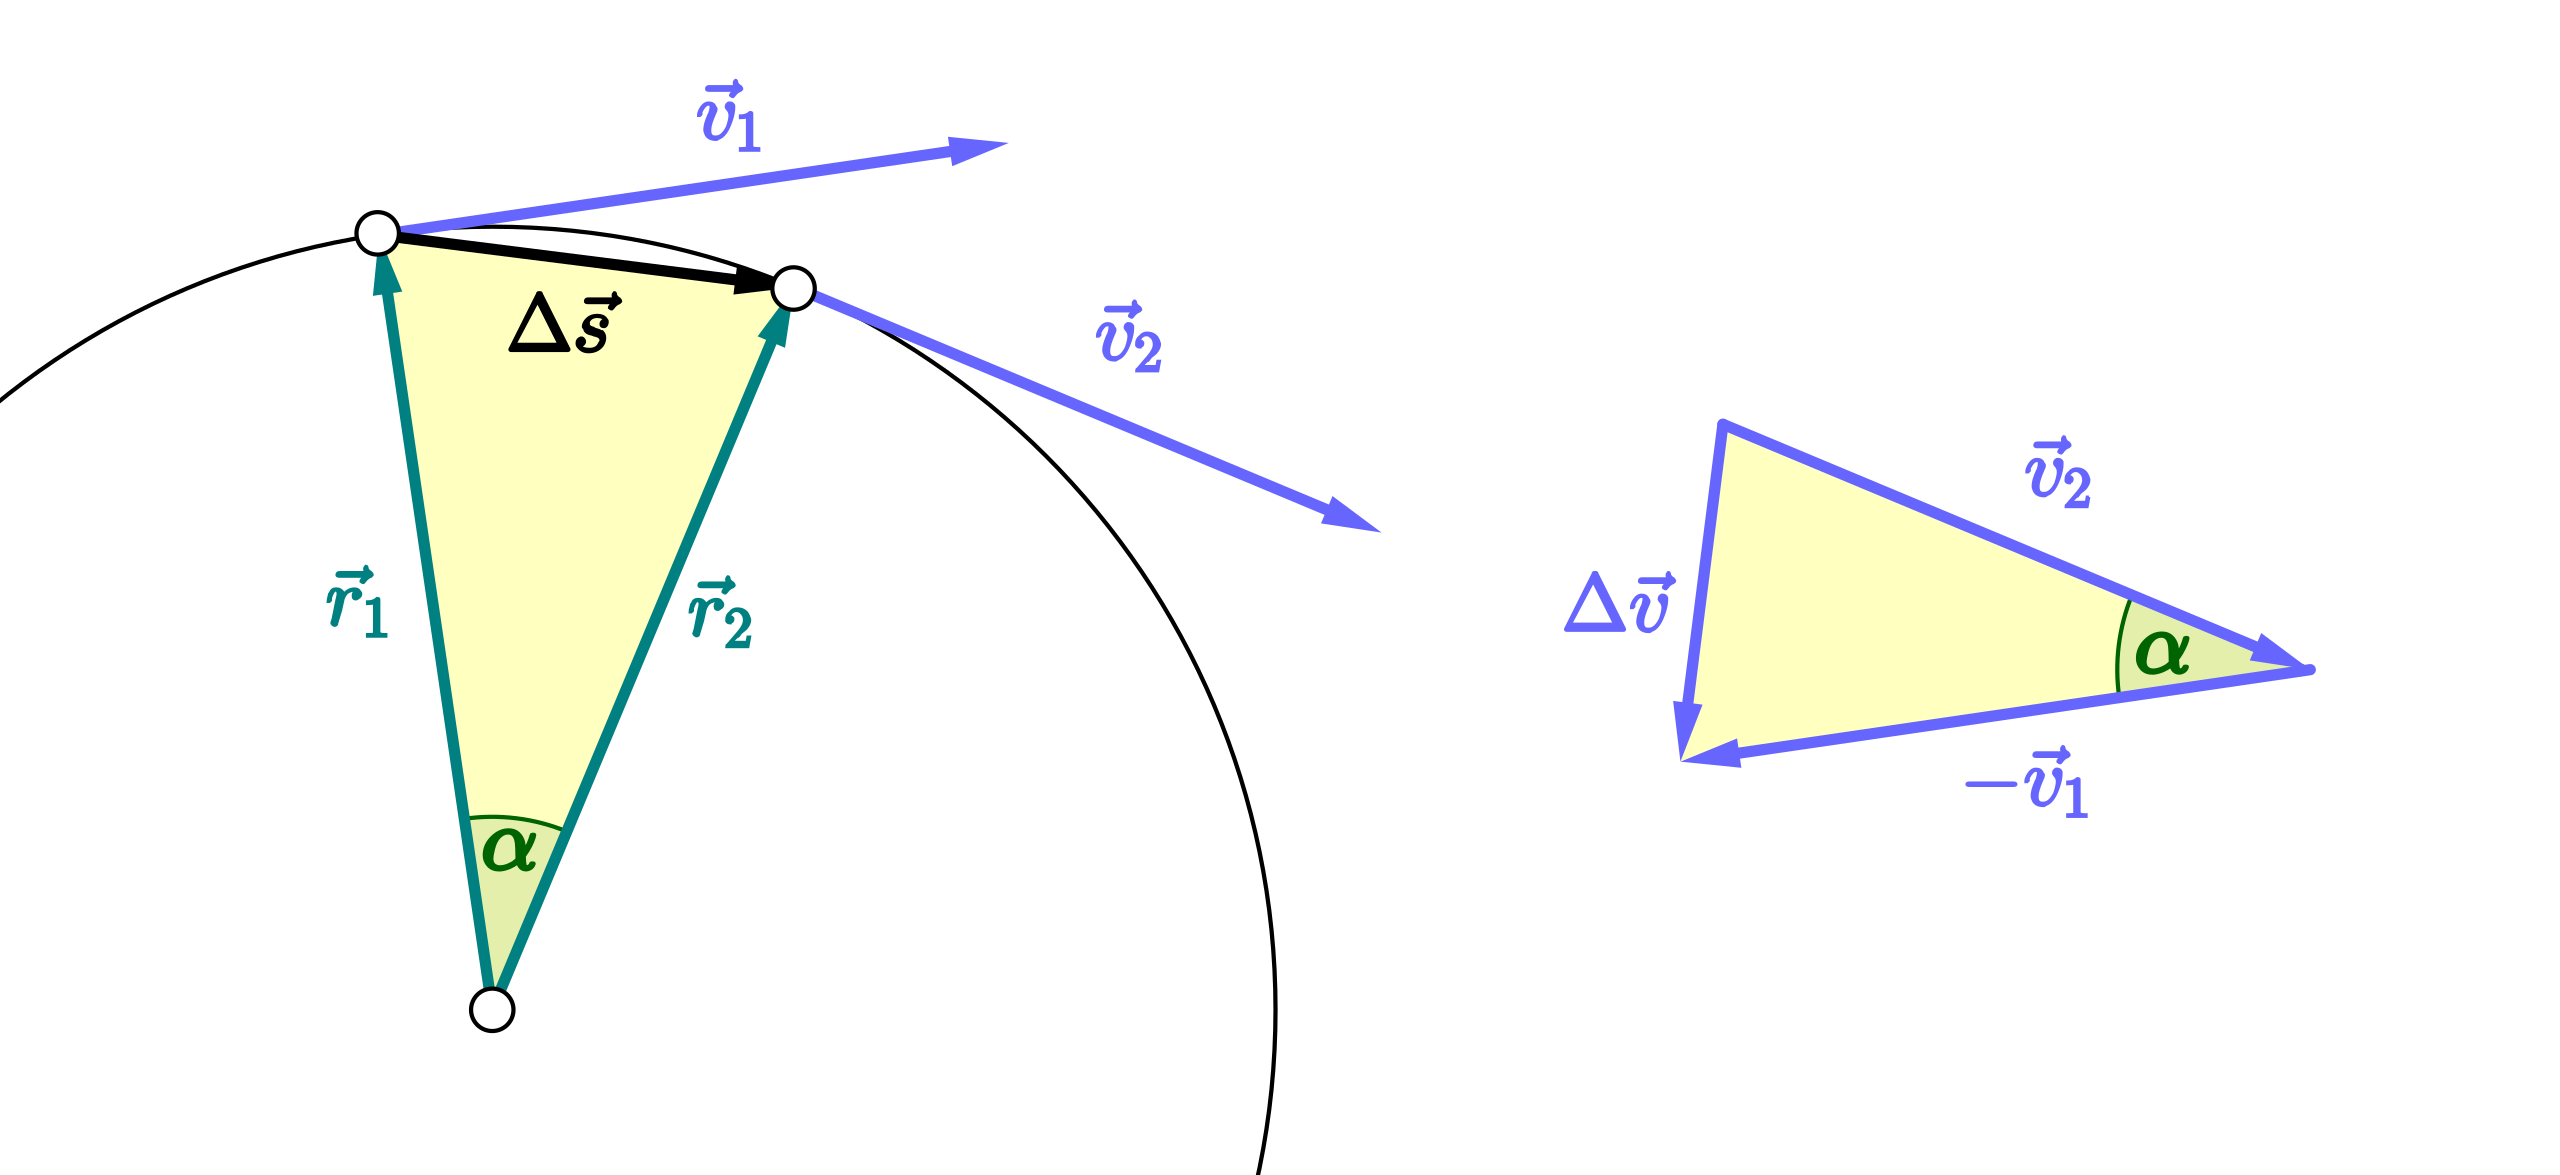
\includegraphics[width=12cm]{Centripetal_acceleration}
\end{figure}
Using similar triangles,
\[ \frac{\Delta s}{r} = \frac{\Delta v}{v} \implies \frac{\Delta s}{\Delta t}\cdot\frac{1}{r} = \frac{\Delta v}{\Delta t}\cdot\frac{1}{v} \]
Taking limits where $\Delta t \to 0$,
\[ \frac{1}{r}\brac{\lim_{\Delta t \to 0}\frac{\Delta s}{\Delta t}} = \frac{1}{v}\brac{\lim_{\Delta t \to 0}\frac{\Delta v}{\Delta t}} \implies \frac{1}{r}\dv{s}{t}=\frac{1}{v}\dv{v}{t} \implies \frac{v}{r} = \frac{a}{v} \implies a = \frac{v^2}{r} \]
\end{proof}
\pagebreak

\subsection{Gravitational Field}
\textbf{Gravitational field strength}
\[ g=-\frac{GM}{r^2} \]
\begin{proof}[Derivation]
Newton's Law of Gravitation states that 
\[ F=-\frac{GMm}{r^2} \]
By the definition of gravitational field strength,
\[ g=\frac{F}{m}=\frac{-\frac{GMm}{r^2}}{m}=-\frac{GM}{r^2} \]
\end{proof}

\textbf{Gravitational field strength near the surface}
\begin{proof}[Derivation]
Consider gravitational field strength at height $h$ above the surface of Earth. Near the surface of Earth, $h$ is small compared to the radius $R$ of Earth, i.e. $h \ll R$.
\[ g = \frac{GM}{(h+R)^2} \approx \frac{GM}{R^2} \]
\end{proof}

\textbf{Gravitational potential energy}
\[ U = -\frac{GMm}{r} \]

\begin{proof}[Derivation]
Consider moving a mass $m$ from infinity to a point at distance $r$ from a mass $M$ at \emph{constant speed} (so that kinetic energy of mass $m$ does not change).

From the definition of gravitational potential energy,
\[ U = \int_{\infty}^r \va{F}_{\mathrm{ext}} \dd{r} \]
Since the external force acts in the opposite direction of gravitational force, $\va{F}_{\mathrm{ext}}=-\va{F}_g$.
\[ U = \int_{\infty}^r -\va{F}_g \dd{r} = \int_{\infty}^r \frac{GMm}{r^2} \dd{r} \]
Computing the integral, 
\[ U = \sqbrac{-\frac{GMm}{r}}^r_{\infty} = -\frac{GMm}{r} \]
\end{proof}
\pagebreak

\subsection{Temperature and Ideal Gases}
\textbf{Kinetic theory of gas}
\[ pV = \frac{1}{3} Nm \langle c^2 \rangle \]
\begin{proof}[Derivation]
Consider an ideal gas consisting of $N$ identical molecules, each of mass $m$, in a cubical container of side length $L$.

Since the molecules move randomly, they do not have any preferred direction of travel along the $x$-, $y$- and $z$-axes. We expect that one-third of the $N$ molecules move along each axis.

Consider a one-dimensional case along the $x$-axis. One gas molecule of mass $m$ approaches and collides elastically with the wall with velocity $c_x$, and leaves the wall with velocity $-c_x$. Change in momentum of gas molecule is given by 
\[ \Delta p = -2mc_x \]

By conservation of linear momentum, wall experiences change in momentum of
\[ \Delta p_\text{wall} = 2mc_x \]

After the collision, assume this molecule continues its motion uninterrupted. It travels a total distance of $2L$ back and forth, and collides with the same wall. The time interval between successive collisions is given by 
\[ \Delta t = \frac{2L}{c_x} \]

Rate of change of momentum of wall due to one molecule is given by 
\[ \frac{\Delta p_\text{wall}}{\Delta t} = -\frac{m{c_x}^2}{L} \]

By Newton's 2nd law, net force on wall is rate of change of momentum of wall due to all $N$ molecules, given by
\begin{align*}
F_\text{wall} &= \frac{m{c_{x1}}^2}{L} + \cdots + \frac{m{c_{xN}}^2}{L} \\
&= \frac{m}{L}\brac{{c_{x1}}^2 + \cdots + {c_{xN}}^2} \\
&= \frac{Nm}{L}\langle {c_x}^2 \rangle
\end{align*}
where mean square speed $\langle {c_x}^2 \rangle$ is defined as
\[ \langle {c_x}^2 \rangle = \frac{{c_{x1}}^2 + \cdots + {c_{xN}}^2}{N} \]

Since the area of the wall is $L^2$, pressure on wall is given by 
\begin{equation*}\tag{1}
p = \frac{F}{L^2} = \frac{Nm}{V}\langle {c_x}^2 \rangle
\end{equation*}
since $V=L^3$.

Applying Pythagoras' Theorem to 3D velocity vector of molecule gives
\[ c^2={c_x}^2+{c_y}^2+{c_z}^2 \implies \langle c^2 \rangle = \langle {c_x}^2 \rangle + \langle {c_y}^2 \rangle + \langle {c_z}^2 \rangle \]

Since there are $\dfrac{N}{3}$ molecules moving along each axis, $\langle {c_x}^2 \rangle = \langle {c_y}^2 \rangle = \langle {c_z}^2 \rangle$. Hence
\[ \langle {c_x}^2 \rangle = \frac{1}{3}\langle c^2 \rangle \]
Substituting this into (1) gives us
\[ pV = \frac{1}{3} Nm \langle c^2 \rangle \]
as desired.
\end{proof}
\begin{remark}
How to remember the derivation:
\begin{itemize}
\item Context, find pressure $P=\frac{F}{A}$
\item Origin of force $F$: collision of one, $N$ gas molecules with wall. Relate rate of change of $\delta p$ to $F=\dv{p}{t}$
\item Generalise for $N$ molecules, apply mean square speed
\end{itemize}
\end{remark}
\begin{remark}
The root mean square is an estimation of a statistical ``average''. Statistically, the \textbf{root mean squared speed} of gas molecules means taking the square root of the sum of the squares of the speeds of all gas molecules.
\[ c_{\text{r.m.s.}} = \sqrt{\frac{{c_1}^2+{c_2}^2+\cdots+{c_n}^2}{n}} \]
\end{remark}
\pagebreak

\subsection{Oscillations}
\textbf{Velocity}
\[ v=\pm\omega\sqrt{{x_0}^2-x^2} \]
\begin{proof}[Derivation]
Displacement is given by
\[ x=x_0\sin\omega t \]
By differentiation, velocity is given by
\[ v=\omega x_0\cos\omega t \]
Using Pythagorean identity $\sin^2 x+\cos^2 x=1$, the given equation can be easily derived.
\end{proof}
\pagebreak

\subsection{Wave Motion}
\textbf{Wave speed}
\[ v=f\lambda \]
\begin{proof}[Derivation]
One wavelength $\lambda$ is distance travelled by wave during one complete oscillation of the source.

Distance travelled by wave during $n$ complete oscillations is $n\lambda$.

Speed of wave is distance per unit time, $v=\dfrac{n\lambda}{t}$.

Frequency is number of oscillations per unit time, $f=\dfrac{n}{t}$.

Hence
\[ f\lambda=\brac{\frac{n}{t}}\lambda=\frac{n\lambda}{t}=v. \]
\end{proof}
\pagebreak

\subsection{Current of Electricity}
\textbf{Transport equation}
\[ I=nAvq \]

\begin{proof}[Derivation]
Consider a current $I$ passing through a section of a wire of cross-sectional area $A$. 

We define
\begin{itemize}
\item $n$ as number density of charge carriers (number per unit volume)
\item $q$ as amount of charge of each charge carrier
\item $v$ as drift velocity of charge carriers
\end{itemize}
\[ I=\frac{Q}{t}=\frac{Nq}{t}=\frac{nVq}{t}=\frac{nAxq}{t}=nAvq \]
\end{proof}
\pagebreak